% 3章
\chapter{数値実験}

研究で新たに実装した歩行者工一ジェントおよび歩車相互作用モデルの定量的な評価性能を検証するために,シミュレーション実験を行った.
この章では,実験で用いた環境設定と,実験結果をどのような評価指標で判断したか,またその結果と考察についてまとめている.

\section{実験条件}

今回の実験では,図\ref{environment}に示すように,15m四方の二次元平面と,排泄場所としてのトイレをその上部に設置した.

\begin{figure}[htb]
\begin{center}
 
\includegraphics[scale=0.6]{figures/environment.png}
 \caption[実験環境]{実験環境 \label{environment}}
\end{center}
\end{figure}

この環境の中で,介護者と被介護者の可視化をおこなっていく.今回の実験では,介護における技術を導入した際に,それが介護環境にどのようなインパクトをあたえるのかについて検証を行うことが目的であるので,介護者の数は1人,被介護者の数は16人と設定し,比較的大きい施設を対象とした.
被介護者のバリエーションとしては,健常者(技術のサポートを受けている被介護者),頻尿である被介護者,認知症等の要因によってトイレにいくというアラートを出すことが難しい状況にある被介護者の3種類を想定している.
それぞれ図\ref{elderly_v1},図\ref{elderly_v2},図\ref{elderly_v3}に示しているように,可視化の際に形を変えることでエージェントがそれぞれどのように相互作用を行っているのかを見ることができる.

\begin{figure}[htb]
\begin{center}
 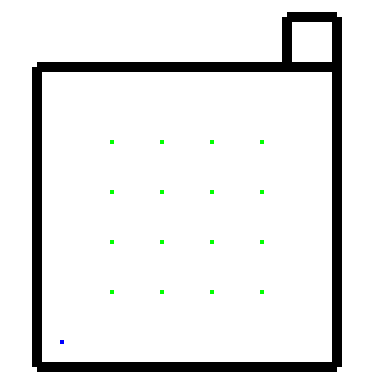
\includegraphics[scale=0.6]{figures/elderly_v1.png}
 \caption[健常者(介護技術を導入した場合の被介護者)の場合の可視化]{健常者(介護技術を導入した場合の被介護者)の場合の可視化 \label{elderly_v1}}
\end{center}
\end{figure}

\begin{figure}[htb]
\begin{center}
 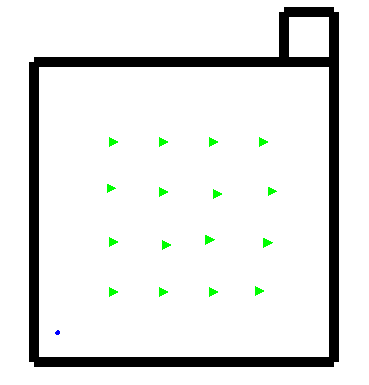
\includegraphics[scale=0.6]{figures/elderly_v2.png}
 \caption[頻尿の場合の可視化]{頻尿の場合の可視化 \label{elderly_v2}}
\end{center}
\end{figure}

\begin{figure}[htb]
\begin{center}
 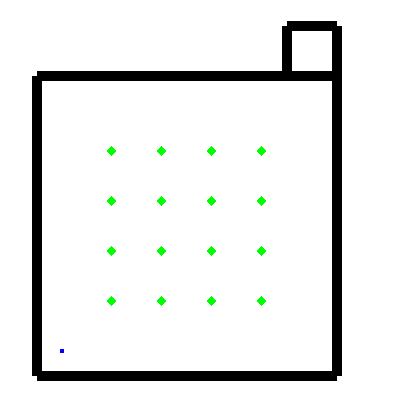
\includegraphics[scale=0.6]{figures/elderly_v3.png}
 \caption[認知症の場合の可視化]{認知症の場合の可視化 \label{elderly_v3}}
\end{center}
\end{figure}

この3種類のエージェントが,介護施設内の自由時間である2時間の間にいかなる回数排泄介助を行うことが必要か,またその介助は本当に必要であったのかということを確かめる実験をおこなう.
一般的に高齢者の排尿量は一回で100-150mlで,1日に8−10回ほどトイレで尿を行うことが知られているので,今回の実験ではそちらの数値を用いることとした.
健常者の場合は,
頻尿の場合は,
認知症の場合は,
この3種類を〜のように組み合わせた6パターンにおいて,相互作用を確認することとする.2時間という時間の中で介護シミュレーションを行い,それを本章で示す評価指標で評価する.

\begin{figure}[htb]
\begin{center}
 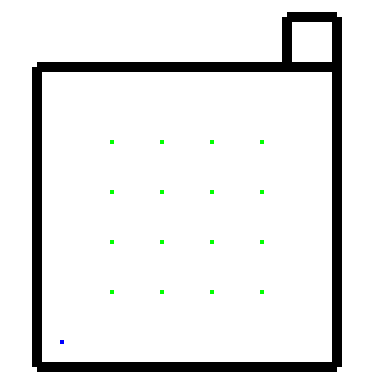
\includegraphics[scale=0.6]{figures/elderly_v1.png}
 \caption[健常者(介護技術を導入した場合の被介護者)の場合の可視化]{健常者(介護技術を導入した場合の被介護者)の場合の可視化 \label{elderly_v1}}
\end{center}
\end{figure}

\begin{figure}[htb]
\begin{center}
 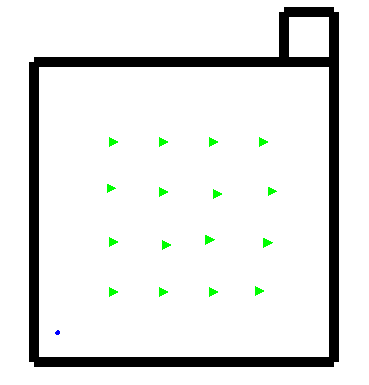
\includegraphics[scale=0.6]{figures/elderly_v2.png}
 \caption[頻尿の場合の可視化]{頻尿の場合の可視化 \label{elderly_v2}}
\end{center}
\end{figure}

\begin{figure}[htb]
\begin{center}
 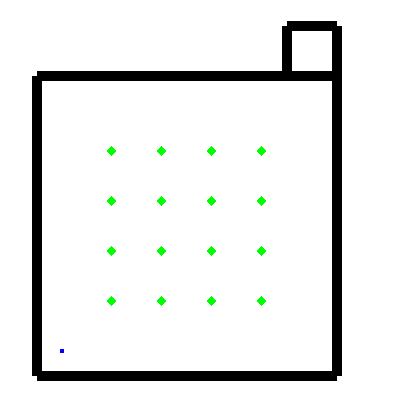
\includegraphics[scale=0.6]{figures/elderly_v3.png}
 \caption[認知症の場合の可視化]{認知症の場合の可視化 \label{elderly_v3}}
\end{center}
\end{figure}

\begin{figure}[htb]
\begin{center}
 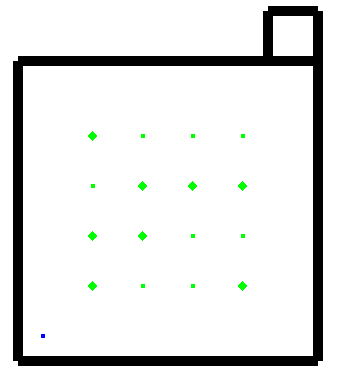
\includegraphics[scale=0.6]{figures/health_urinate.png}
 \caption[健常者と認知症の場合の可視化]{健常者と認知症の場合の可視化 \label{health_urinate}}
\end{center}
\end{figure}

\begin{figure}[htb]
\begin{center}
 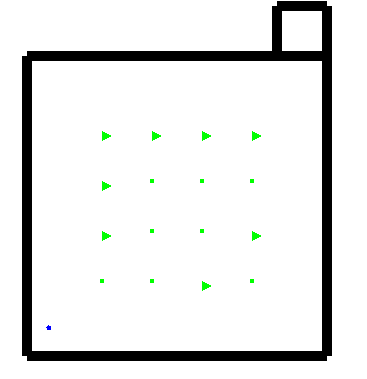
\includegraphics[scale=0.6]{figures/health_frequently_urinate_v1.png}
 \caption[健常者と頻尿の場合の可視化]{健常者と頻尿の場合の可視化 \label{health_frequently_urinate_v1}}
\end{center}
\end{figure}

\begin{figure}[htb]
\begin{center}
 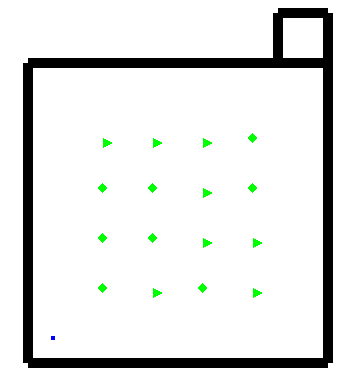
\includegraphics[scale=0.6]{figures/dementia_urinate_v1.png}
 \caption[認知症と頻尿の場合の可視化]{認知症と頻尿の場合の可視化 \label{dementia_urinate_v1}}
\end{center}
\end{figure}

Case1は、健常の被介護者(技術の補助を受けた被介護者)が100%の状態,Case2は頻尿の被介護者が100%の状態,Case3は認知症の被介護者が100%の状態,Case4は、健常の被介護者(技術の補助を受けた被介護者)と頻尿の被介護者が50%ずつの状態,Case5は健常の被介護者(技術の補助を受けた被介護者)と認知症の被介護者が50%ずつの状態,Case6は頻尿の被介護者と認知症の被介護者が50%ずつの状態を表現し,それぞれで実験を行う.実験条件については表\ref{experiment}に示す.

\begin{table}[htb]
  \caption[実験条件]{実験条件}
  \label{experiment}
  \centering
  \begin{tabular}{r|c|c|c|c|c|c}
     & Case1 & Case2 & Case3 & Case4 & Case5 & Case6 \\ \hline
    健常者 & 100% & 0% & 0% & 50% & 50% & 0% \\
    頻尿   & 0% & 100% & 0% & 50% & 0% & 50% \\
    認知症 & 0% & 0% & 100% & 0% & 50% & 50% \\
    \end{tabular}
\end{table}

\section{介護挙動の基本的な検証}

本シミュレータが現実を反映できているのかについて,簡単な検証を行った.
被介護者が,時系列で尿量が加算されて行き,その数値が健常者の場合は100mlを超えた時点で,頻尿の被介護者は〜を超えた時点で,認知症の被介護者は〜を超えた時点で,トイレに行きたいというアラートを発するように内部状態を設定した.その結果,健常者の場合は,2時間の間に1回トイレに行くという結果を得ることができた.これは実際のデータと比較しても整合性のある値となった.この結果を表\ref{number_of_urination}に示す.なお,実験では16人の被介護者が存在するので実際は数値を16で割った数字が一人当たりの回数となっている.

\begin{table}[htb]
  \caption[被介護者ごとの排尿回数]{被介護者ごとの排尿回数}
  \label{number_of_urination}
  \centering
  \begin{tabular}{r|c|c|c}
     & 健常者 & 頻尿 & 認知症 \\ \hline
    一回目 & 15 & 21 & 6 \\
    二回目 & 15 & 22 & 5 \\
    三回目 & 16 & 26 & 5 \\
    \end{tabular}
\end{table}

\section{評価指標}

本研究の目的は,疾患のある被介護者,すなわち現状介護者の負担増の原因となっており,被介護者自身も自らの排泄が負担となっているようなケースにおいて,技術の導入を行うことでどれだけの効果が得られるのかを可視化するというものである.そこで,評価指標としては,排泄に行くべきである尿量の状態,あるいは自身が排泄に行きたいと感じている状態から実際に排泄を行うまでの時間を計測し,それを総我慢時間とし,本研究の評価指標とする.

\section{結果および考察}

図\ref{result_v1}に,介護者・被介護者の割合をそれぞれ変化させた場合のシミュレーション結果(10回の試行の平均値)を示す.

\begin{figure}[htb]
\begin{center}
 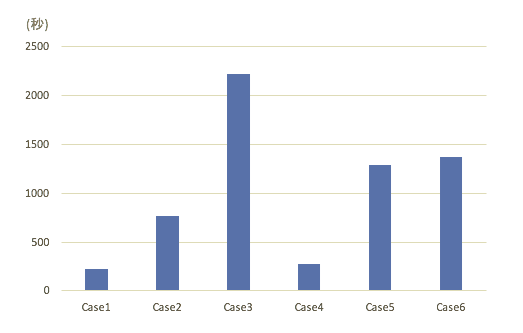
\includegraphics[scale=0.6]{figures/result_1.png}
 \caption[実験結果]{実験結果 \label{result_v1}}
\end{center}
\end{figure}
